% \setchapterpreamble[u]{\margintoc}
\chapter{Streams, Redirections, Piping}
\labch{redirection}

\section{Multiple Commands in a Single Line}

Sometimes we may want to run multiple commands in a single line.
For example, we may want to run two commands \lstinline|ls| and \lstinline|wc|
in a single line. We can do this by separating the commands with a semicolon.
This helps us see the output of both the commands without having the
prompt in between.

For example, the following command will run \lstinline|ls| and \lstinline|wc| in a single line.

\begin{lstlisting}[language=bash]
$ ls; wc .bashrc
docs  down  music  pics  programs  scripts  tmp  vids
  340  1255 11238 .bashrc
\end{lstlisting}

In this way of executing commands, the success or failure of one
command does not affect the other command. Concisely, the commands
are executed independently and sequentially. Even if a command
fails, the next command will be executed.

\begin{lstlisting}[language=bash]
$ date; ls /nonexistant ; wc .bashrc
Wed Jul  3 06:54:45 PM IST 2024
ls: cannot access '/nonexistant': No such file or directory
  340  1255 11238 .bashrc
\end{lstlisting}

\subsection{Conjunction and Disjunction}

We can also run multiple commands in a single line using conjunction
and disjunction. The conjunction operator \lstinline|&&| is used to run
the second command only if the first command is successful. The disjunction
operator \lstinline|||| is used to run the second command only if the first
command fails. In computer science, these operators are also known as
short-circuit logical \textbf{AND} and \textbf{OR} operators.
\sidenote{
  A short-circuit logical \textbf{AND} operator returns \textbf{true}
  if both the operands are \textbf{true}. If the first operand is \textbf{false},
  it does not evaluate the second operand and returns \textbf{false} directly.
}

\begin{lstlisting}[language=bash]
$ ls /nonexistant && echo "ls successful"
ls: cannot access '/nonexistant': No such file or directory
$ ls /home && echo "ls successful"
lost+found  sayan  test1
ls successful
\end{lstlisting}

In the first command, the \lstinline|ls| command fails, so the \lstinline|echo|
command is not executed. In the second command, the \lstinline|ls| command
is successful, so the \lstinline|echo| command is executed.

The success or failure of a command is determinted by the exit status
of the command. If the exit status is 0, the command is successful.
If the exit status is non-zero, the command is considered to have failed.

The exit status of the last command can be accessed using the special
variable \lstinline|$?|. This variable contains the exit status of the
last command executed.

\begin{lstlisting}[language=bash]
$ ls /nonexistant
ls: cannot access '/nonexistant': No such file or directory
$ echo $?
2
\end{lstlisting}

Here, the exit status of the \lstinline|ls| command is 2, because the
file \lstinline|/nonexistant| does not exist.

\begin{lstlisting}[language=bash]
$ ls /home
lost+found  sayan  test1
$ echo $?
0
\end{lstlisting}

Here, the exit status of the \lstinline|ls| command is 0, because the
directory \lstinline|/home| exists, and the command is successful.

Similarly, we can use the disjunction operator \lstinline|||| to run
the second command only if the first command fails.

\begin{lstlisting}[language=bash]
$ ls /nonexistant || echo "ls failed"
ls: cannot access '/nonexistant': No such file or directory
ls failed
\end{lstlisting}

In this case, the \lstinline|ls| command fails, so the \lstinline|echo|
command is executed. However, since the disjunction operator is a
short-circuit operator, the \lstinline|echo| command is executed only
if the \lstinline|ls| command fails. If the \lstinline|ls| command is
successful, the \lstinline|echo| command is not executed.

\begin{lstlisting}[language=bash]
$ ls /home || echo "ls failed"
lost+found  sayan  test1
\end{lstlisting}

In this case, the \lstinline|ls| command is successful, so the \lstinline|echo|
command is not executed.

We can also chain multiple commands using conjunction and disjunction.

\begin{lstlisting}[language=bash]

$ date && ls /hello || echo "echo"
Thu Jul  4 06:53:08 AM IST 2024
ls: cannot access '/hello': No such file or directory
echo
\end{lstlisting}

In this case, the \lstinline|date| command is successful, so the \lstinline|ls|
is executed. The \lstinline|ls| command fails, so the \lstinline|echo| command
is executed.

However, even if the first command fails, and the second command is
skipped, the third command is executed.

\begin{lstlisting}[language=bash]
$ ls /hello && date || echo echo
ls: cannot access '/hello': No such file or directory
echo
\end{lstlisting}

In this case, the \lstinline|ls| command fails, so the \lstinline|date| command
is not executed. However, the \lstinline|echo| command is executed as the
exit status of the \lstinline|ls| command is non-zero.

To make the \lstinline|echo| command execute only if the \lstinline|date|
command is run and fails, we can use parentheses.

\begin{lstlisting}[language=bash]
$ ls /hello && (date || echo echo)
ls: cannot access '/hello': No such file or directory
\end{lstlisting}

Although the parentheses look like grouping a mathematical expression,
they are actually a subshell. The commands inside the parentheses
are executed in a subshell. The exit status of the subshell is the
exit status of the last command executed in the subshell.

We can see the subshell count using the \lstinline|echo \$BASH\_SUBSHELL|.

\begin{lstlisting}[language=bash]
$ echo $BASH_SUBSHELL
0
$ (echo $BASH_SUBSHELL)
1
$ (:;(echo $BASH_SUBSHELL ))
2
$ (:;(:;(echo $BASH_SUBSHELL )))
3
\end{lstlisting}

\begin{remark}
  When nesting in more than one subshell, simply putting two parentheses
  side by side will not work. This is because the shell will interpret
  that as the mathematical evaluation of the expression inside the
  parentheses. To avoid this, we can use a colon \lstinline|:| no-op command
  followed by a semicolon \lstinline|;| to separate the two parentheses.
\end{remark}

\begin{remark}
  Setting up an environment takes up time and resources. Thus, it is
  better to avoid creating subshells unless necessary.
\end{remark}

\vfill
\pagebreak
\section{Streams}

There are three standard streams in Unix-like operating systems:

\begin{enumerate}
  \item \textbf{Standard Input (stdin)}: This is the stream where the
    input is read from. By default, the standard input is the keyboard.
  \item \textbf{Standard Output (stdout)}: This is the stream where the
    output is written to. By default, the standard output is the terminal.
  \item \textbf{Standard Error (stderr)}: This is the stream where the
    error messages are written to. By default, the standard error is the
    terminal.
\end{enumerate}

There are also other numbered streams, such as \lstinline|3|, \lstinline|4|,
etc., which can be used to read from or write to files.

\begin{marginfigure}
  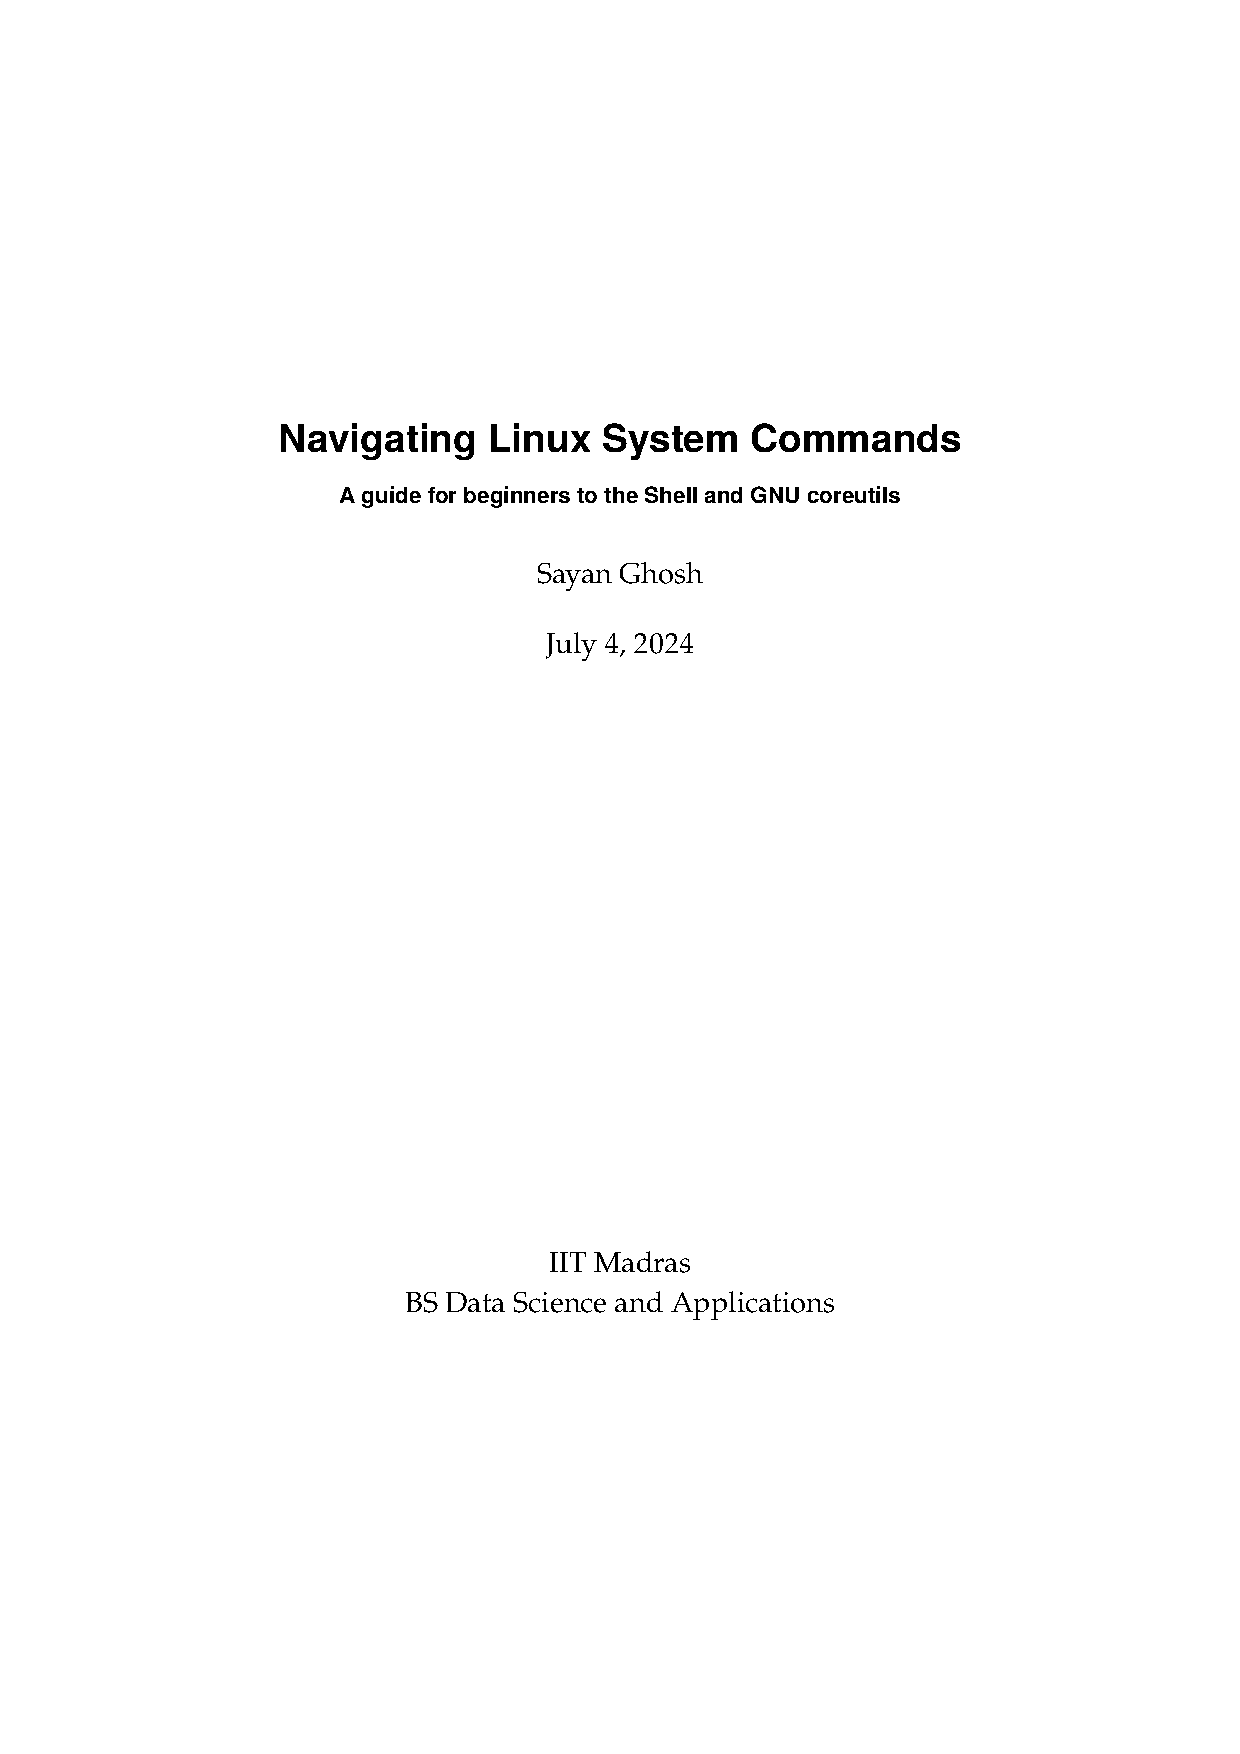
\includegraphics{streams}
  \caption{Standard Streams}
  \labfig{streams}
\end{marginfigure}

However, sometimes a process may need to take input from a file or
send output to a file. When this is required, the standard stream is
mapped to a file. This is known as \textbf{redirection}.

To maintain which file or resource is mapped to which stream, the
operating system maintains a table known as the \textbf{file descriptor
table}. The file descriptor table is a table that maps the file
descriptors to the files or resources.

\begin{definition}[File Descriptor]
  A \textbf{file descriptor} is a process-unique identifier that the
  operating system assigns to a file or resource.
  The file descriptor is an integer that is used to identify
  the file or resource.
\end{definition}

The default file descriptors are:

\begin{enumerate}
  \item \textbf{Standard Input (stdin)}: File descriptor 0
  \item \textbf{Standard Output (stdout)}: File descriptor 1
  \item \textbf{Standard Error (stderr)}: File descriptor 2
\end{enumerate}

In the traditional implementation of Unix, file descriptors index
into a per-process file descriptor table maintained by the kernel,
that in turn indexes into a system-wide table of files opened by
all processes, called the file table. This table records the mode
with which the file (or other resource) has been opened: for
reading, writing, appending, and possibly other modes. It also indexes
into a third table called the inode table
\sidenote{
  We have covered inodes and inode tables in detail in the
  \refch{basic} chapter.
}
that describes the actual
underlying files. To perform input or output, the process passes
the file descriptor to the kernel through a system call, and the
kernel will access the file on behalf of the process. The process
does not have direct access to the file or inode tables.

\begin{marginfigure}
  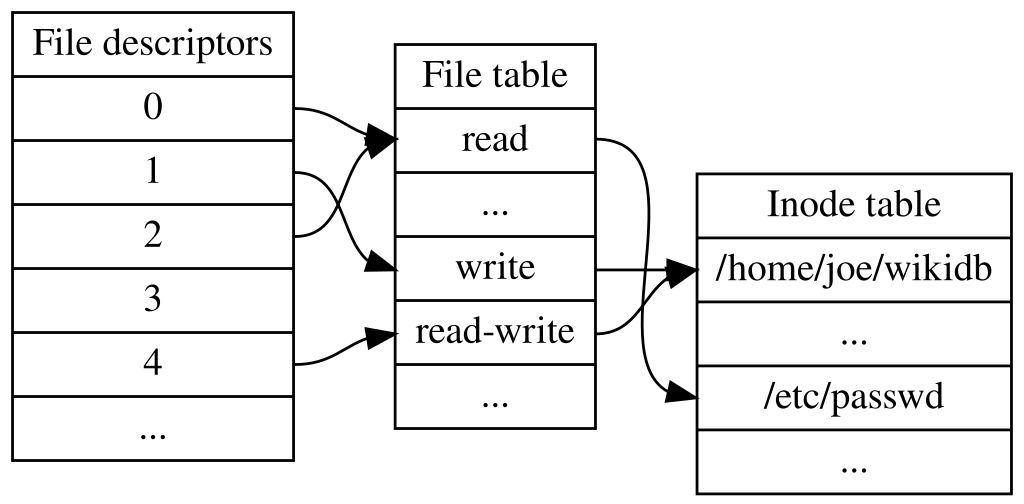
\includegraphics{fdtable}
  \caption{File Descriptor Table}
  \labfig{fdtable}
\end{marginfigure}

The file descriptors of a process can be inspected in the \lstinline|/proc|
directory. The \lstinline|/proc| directory is a pseudo-filesystem that
provides an interface to kernel data structures. The \lstinline|/proc/PID/fd|
directory contains the file descriptors of the process with the PID.

Most GNU core utilities that accept a file as an argument will also
work without the argument and will read from the standard input.
This behaviour lets us chain commands together using pipes easily
without any explicit file handling.

\begin{lstlisting}[language=bash]
$ cat
hello
hello
This command is repeating the input
This command is repeating the input
Press Ctrl+D to exit
Press Ctrl+D to exit
\end{lstlisting}

The \lstinline|cat| command is usually used to print the contents of one
or more files. However, when no file is provided, it reads from the
standard input. In this case, the standard input is the keyboard.
This is very useful when we want to repeat the input or when we want
to read from the standard input.

\begin{qs}
  Can we also use cat to write to a file?
\end{qs}

\begin{ans}
  Yes, we can use the \lstinline|cat| command to write to a file. When
  no file is provided, the \lstinline|cat| command reads from the standard
  input. So the input will be printed back to the standard output.
  However, if we can somehow change the standard output to a file,
  then the input will be written to the file.
\end{ans}

\section{Redirection}

Redirection is the process of changing the standard streams of a process.
This is done by the shell before the process is executed. The shell
uses the \lstinline|<|, \lstinline|>|, and \lstinline|2>| operators to redirect
the standard input, standard output, and standard error streams of a
process.

As the shell is responsible for redirection, the process is not aware
of the redirection. The process reads from or writes to the file descriptor
it is given by the shell. The process does not know whether the file
descriptor is a file, a terminal, or a pipe.

However, there are ways for a process to guess whether the file descriptor
is a terminal or a file. This is done by using the \lstinline|isatty()|
function. The \lstinline|isatty()| function returns \lstinline|1| if the file
descriptor is a terminal, and \lstinline|0| if the file descriptor is a file.

\subsection{Standard Output Redirection}

The standard output of a process can be redirected to a file using the
\lstinline|>| operator. Observe the following example.

\begin{lstlisting}[language=bash]
$ date > date.txt
$ cat date.txt
Thu Jul  4 07:37:27 AM IST 2024
\end{lstlisting}

Here, the output of the \lstinline|date| command is redirected to the file
\lstinline|date.txt|. The \lstinline|cat| command is then used to print the
contents of the file \lstinline|date.txt|.

The process did not print the output to the terminal. Instead, the shell
changed the standard output of the process to the file \lstinline|date.txt|.

We can also use redirection to create a file. If the file does not exist,
the shell will create the file. If the file exists, the shell will truncate
the file.

\begin{lstlisting}[language=bash]
$ > empty.txt
\end{lstlisting}

This command creates an empty file \lstinline|empty.txt|. The \lstinline|>|
operator is used to redirect the output of the command to the file
\lstinline|empty.txt|. Since there is no output, the file is empty.

We can also use redirection along with the \lstinline|echo| command to
create a file with some content.

\begin{lstlisting}[language=bash]
$ echo "hello" > hello.txt
$ cat hello.txt
hello
\end{lstlisting}

Here, the output of the \lstinline|echo| command is redirected to the file
\lstinline|hello.txt|. The \lstinline|cat| command is then used to print the
contents of the file \lstinline|hello.txt|.

Recall that the cat command will read from the standard input if no
file is provided. We can use this to create a file with the input from
the standard input.

\begin{lstlisting}[language=bash]
$ cat > file.txt
hello, this is input typed from the keyboard
I am typing more input
all this is being written to the file
to stop, press Ctrl+D
$ cat file.txt
hello, this is input typed from the keyboard
I am typing more input
all this is being written to the file
to stop, press Ctrl+D
\end{lstlisting}

It is important to note that the process of creating the file if it
does not exist, and truncating the file if it exists, along with redirecting
the output, is done by the shell, not the process. All of this is done
before the process is executed. This creates an interesting exemplar when
using redirection with the \lstinline|ls| command.

\textbf{Output contains output}

\begin{lstlisting}[language=bash]
$ ls
hello
$ ls > output.txt
$ cat output.txt
hello
output.txt
\end{lstlisting}

Since the file is created even before the process is executed, the file
is also a part of the output of the \lstinline|ls| command. This is why the
file \lstinline|output.txt| is also printed by the \lstinline|cat| command.

\textbf{Output format changes}

Another interesting example using the \lstinline|ls| command is when the
directory contains more than one file.
The output of \lstinline|ls| is usually formatted to fit the terminal.
However, when the output is redirected to a file, the output is not
in a column format. Instead, each file is printed on a new line.

\begin{lstlisting}[language=bash]
$ ls
hello  output.txt
$ ls > output.txt
$ cat output.txt
hello
output.txt
\end{lstlisting}

Observe that the output of the \lstinline|ls| command is not in a column
when redirected to a file. But how does \lstinline|ls| know that the output
is not a terminal? It uses the file descriptor to guess whether the
output is a terminal or a file. If the file descriptor is a terminal,
then the output is formatted to fit the terminal. If the file descriptor
is a file, then the output is not formatted.

However, we can always force the output to be single-column using the
\lstinline|-1| option.

\begin{lstlisting}[language=bash]
$ ls -1
hello
output.txt
\end{lstlisting}

This behaviour is not limited to the \lstinline|ls| command. Most commands
usually strip out the formatting when the output is redirected to a file.

If you are using a terminal that supports ANSI escape codes
\sidenote{
  ANSI escape codes are special sequences of characters that are used
  to control the terminal. For example, to change the color of the text,
  the ANSI escape code \lstinline|\[31m| is used.
  Similarly other ANSI escape codes are used to change the text style,
  and the position and state of the cursor.
}
, you can
use the \lstinline|ls| command with the \lstinline|--color=auto| option to
get colored output. However, when the output is redirected to a file,
the ANSI escape codes are not printed. This is because the ANSI escape
codes are not printable characters. They are control characters that
tell the terminal to change the color of the text.

\textbf{Output and Input from same file}

If you try to redirect the output of a command to a file, and then
also try to read from the same file, you will get an empty file.
This is because the file is truncated before the command is executed.

\begin{lstlisting}[language=bash]
$ echo "hello" > output.txt
$ cat output.txt
hello
$ cat output.txt > output.txt
$ cat output.txt
$
\end{lstlisting}

\begin{remark}
  Although we can simply use \lstinline|>| to redirect the output to a file,
  the full syntax is \lstinline|1>|. This is because the file descriptor
  for the standard output is 1. The \lstinline|1>| is used to redirect
  the standard output to a file. However, since the standard output
  is the default output, we can omit the \lstinline|1| and use only \lstinline|>|.
\end{remark}

\subsection{Standard Error Redirection}

The standard error of a process can be redirected to a file using the
\lstinline|2>| operator. Observe the following example.

\begin{lstlisting}[language=bash]
$ ls /nonexistant 2> error.txt
$ cat error.txt
ls: cannot access '/nonexistant': No such file or directory
\end{lstlisting}

Here, the error message of the \lstinline|ls| command is redirected to the
file \lstinline|error.txt|. The \lstinline|cat| command is then used to print
the contents of the file \lstinline|error.txt|.

It is important to realise that each process has two streams to output
to, the standard output and the standard error. The standard output is
usually used to print the output of the process, while the standard error
is used to print the error messages.

This helps us differentiate between the output and the error messages.
Also, if the output of a process is redirected to a file, the error
will still be printed to the terminal. This is because the standard
error is not redirected to the file. This makes debugging easier, as
the error messages are not lost.

\begin{lstlisting}[language=bash]
$ ls -d /home /nonexistant > output.txt
ls: cannot access '/nonexistant': No such file or directory
$ cat output.txt
/home
\end{lstlisting}

Here, the output of the \lstinline|ls| command is redirected to the file
\lstinline|output.txt|. However, the error message is still printed to
the terminal.

We can redirect both the standard output and the standard error to
files using the \lstinline|>| and \lstinline|2>| operators.

\begin{lstlisting}[language=bash]
$ ls -d /home /nonexistant > output.txt 2> error.txt
$ cat output.txt
/home
$ cat error.txt
ls: cannot access '/nonexistant': No such file or directory
\end{lstlisting}

\textbf{Redirecting both streams to the same file}

Lets try to redirect both the standard output and the standard error
to the same file.

\begin{lstlisting}[language=bash]
$ ls -d /home /nonexistant > output.txt 2> output.txt
$ cat output.txt
/home
nnot access '/nonexistant': No such file or directory
\end{lstlisting}

Why did the error message get mangled? This is because the shell
truncates the file before the process is executed. So the error
is written to the file, and then the output message is written to
the same file, overwriting the error partially.
Observe that only the first six characters of the
error message are mangled, the same size of the output.
\sidenote{
  The output message is \lstinline|/home|, followed by a newline character.
  This makes the output message 6 characters long.
  The shell first writes the error message to the file (because that is
  printed first by the ls command), and then overwrites the first 6 bytes
  of the file with the output message. Since the 6th byte is a newline
  character, it looks like there are two lines in the file.
}

The correct way to redirect both the standard output and the standard
error to the same file is to use the \lstinline|2>\&1| operator.
This means that the standard error is redirected to the standard output.
Here, the \lstinline|1| is the file descriptor for the standard output.
The \lstinline|&| is used to tell the shell that the \lstinline|1| is a file
descriptor, not a file.

\begin{lstlisting}[language=bash]
$ ls -d /home /nonexistant > output.txt 2>&1
$ cat output.txt
ls: cannot access '/nonexistant': No such file or directory
/home
\end{lstlisting}

However, the order is important. The \lstinline|2>\&1| operator should
be placed at the end of the command. If it is placed at the beginning,
then the standard error will be redirected to the standard output, which,
at that point, is the terminal. Then the standard output will be redirected
to the file. Thus, only the standard output will be redirected to the file.

\begin{lstlisting}[language=bash]
$ ls -d /home /nonexistant 2>&1 > output.txt
ls: cannot access '/nonexistant': No such file or directory
$ cat output.txt
/home
\end{lstlisting}

\subsection{Appending to a File}

The \lstinline|>| operator is used to redirect the output to a file. If the
file does not exist, the shell will create the file. If the file exists,
the shell will truncate the file. However, if we want to append the output
to the file, we can use the \lstinline|>>| operator.

\begin{lstlisting}[language=bash]
$ echo "hello" > hello.txt
$ cat hello.txt
hello
$ echo "world" > hello.txt
$ cat hello.txt
world
$ echo "hello" > hello.txt
$ echo "world" >> hello.txt
$ cat hello.txt
hello
world
\end{lstlisting}

Observe that the \lstinline|>| operator truncates the file, while the
\lstinline|>>| operator appends to the file.

We can also append the standard error to a file using the \lstinline|2>>|

\begin{lstlisting}[language=bash]
$ ls /nonexistant 2> error.txt
$ cat error.txt
ls: cannot access '/nonexistant': No such file or directory
$ daet 2>> error.txt
$ cat error.txt
ls: cannot access '/nonexistant': No such file or directory
bash: daet: command not found
\end{lstlisting}

This is useful when we want to append the error messages to a file,
like in a log file.

\textbf{Circular Redirection}

If we try to redirect the output of a command to the same file that
we are reading from, we will get an empty file. However, if we append
the output to the file, we will get an infinite loop of the output.
This should not be done, as it will fill up the disk space.
However, GNU core utilities \lstinline|cat| is smart enough to detect
this and will not read from the file.

\begin{lstlisting}[language=bash]
$ echo hello > hello
$ cat hello >> hello
cat: hello: input file is output file
$ cat < hello > hello
cat: -: input file is output file
\end{lstlisting}

However, it can still be tricked by using a pipe.
\sidenote{
  We will cover pipes in the next section.
}

\begin{lstlisting}[language=bash]
$ echo hello > hello
$ cat hello | cat >> hello
$ cat hello
hello
hello
\end{lstlisting}

Here we dont get into an infinite loop because the first cat command
reads from the file and writes to the pipe. The second cat command
reads from the pipe and writes to the file. Since the file is not
read from and written to at the same time, we dont get into an infinite
loop.

However, BSD utilities like \lstinline|cat| do not have this check, thus
giving the same input and output file will result in an infinite loop.

\subsection{Standard Input Redirection}

The standard input of a process can be redirected from a file using
the \lstinline|<| operator. Although most commands accept a filename
in the argument to read from, so we can directly provide the file
in the argument. However, some commands do not accept a filename
and only read from the standard input. In such cases, we can use
the \lstinline|<| operator to redirect the standard input from a file.

\begin{lstlisting}[language=bash]
$ wc < ~/.bashrc
  340  1255 11238
\end{lstlisting}

Although the \lstinline|wc| command accepts a filename as an argument,
we can also redirect the standard input from a file using the \lstinline|<|
to the command. However, now the output of the \lstinline|wc| command
is different than when we provide the filename as an argument.

\begin{lstlisting}[language=bash]
$ wc ~/.bashrc
  340  1255 11238 /home/sayan/.bashrc
\end{lstlisting}

When we provide the filename as an argument, the \lstinline|wc| command
prints the number of lines, words, and characters in the file, followed
by the filename. However, when we redirect the standard input from a
file, the \lstinline|wc| command prints only the number of lines, words,
and characters in the file. This is because it does not know that the
input is coming from a file. For \lstinline|wc|, the input is just a stream
coming from the standard input.

\begin{lstlisting}[language=bash]
$ wc
Hello, this is input from the keyboard
I can simply type more input here
All of this is taken as standard input
by wc command
Stop by pressing Ctrl+D
      5      29     150
\end{lstlisting}

Another example where giving filename is not possible is the \lstinline|read|
command. The \lstinline|read| command reads a line from the standard input
and assigns it to a variable. The \lstinline|read| command does not accept
a filename as an argument. So we have to use the \lstinline|<| operator to
redirect the standard input from a file.

\begin{lstlisting}[language=bash]
$ read myline < /etc/hostname
$ echo $myline
rex
\end{lstlisting}

Here, the \lstinline|read| command reads a line from the file \lstinline|/etc/hostname|
and assigns it to the variable \lstinline|myline|. The \lstinline|echo| command
is then used to print the value of the variable \lstinline|myline|.
To access the value of the variable, we use the \lstinline|$| operator.
\sidenote{
  This will be covered in depth in the \refch{variables} chapter.
}

\subsection{Here Documents}

A \textbf{here document} is a way to provide input to a command without
using a file. The input is provided directly in the command itself.
This is done by using the \lstinline|<<| operator followed by a delimiter.

\begin{lstlisting}[language=bash]
$ wc <<EOF
This is acting like a file
however the input is directly provided
to the shell or the script
this is mostly used in scripts
we can use any delimiter instead of EOF
to stop, type the delimiter on a new line
EOF
      6      41     206
\end{lstlisting}

We can optionally provide a hyphen \lstinline|-| after the \lstinline|<<|
to ignore leading tabs. This is useful when the here document is
indented.

\begin{lstlisting}[language=bash]
$ cat <<EOF
> hello
>     this is space
>       this is tab
> EOF
hello
    this is space
        this is tab
$ cat <<-EOF
hello
    this is space
        this is tab
EOF
hello
    this is space
this is tab
\end{lstlisting}

The delimiter can be any string. However, it is common to use \lstinline|EOF|
as the delimiter. The delimiter should be on a new line.

\begin{lstlisting}[language=bash]
$ wc <<END
If I want to have
EOF
as part of the input
then I can simply change the delimiter
END
      4      18      82
\end{lstlisting}

Here-documents also support variable expansion. The shell will expand
the variables before passing the input to the command. Thus
it is really useful in scripts if we want to provide a template
which is filled with the values of the variables.

\begin{lstlisting}[language=bash]
$ name="Sayan"
$ cat <<EOF
Hello, $name
This is a here document
EOF
Hello, Sayan
This is a here document
\end{lstlisting}

\subsection{Here Strings}

A \textbf{here string} is a way to provide input to a command without
using a file. The input is provided directly in the command itself.
This is done by using the \lstinline|<<<| operator followed by the input.
It is very similar to the here document, but the input is provided
in a single line. Due to this, a delimiter is not required.

\begin{lstlisting}[language=bash]
$ wc <<< "This is a here string"
      1       5      22
\end{lstlisting}

It can also perform variable expansion.

\begin{lstlisting}[language=bash]
$ cat <<< "Hello, $USER"
Hello, sayan
\end{lstlisting}

\begin{remark}
  Both heredocs and herestrings are simply syntactic sugar. They are
  similar to using echo and piping the output to a command. However,
  it requires one less process to be executed.
\end{remark}

\section{Pipes}

\begin{marginfigure}
  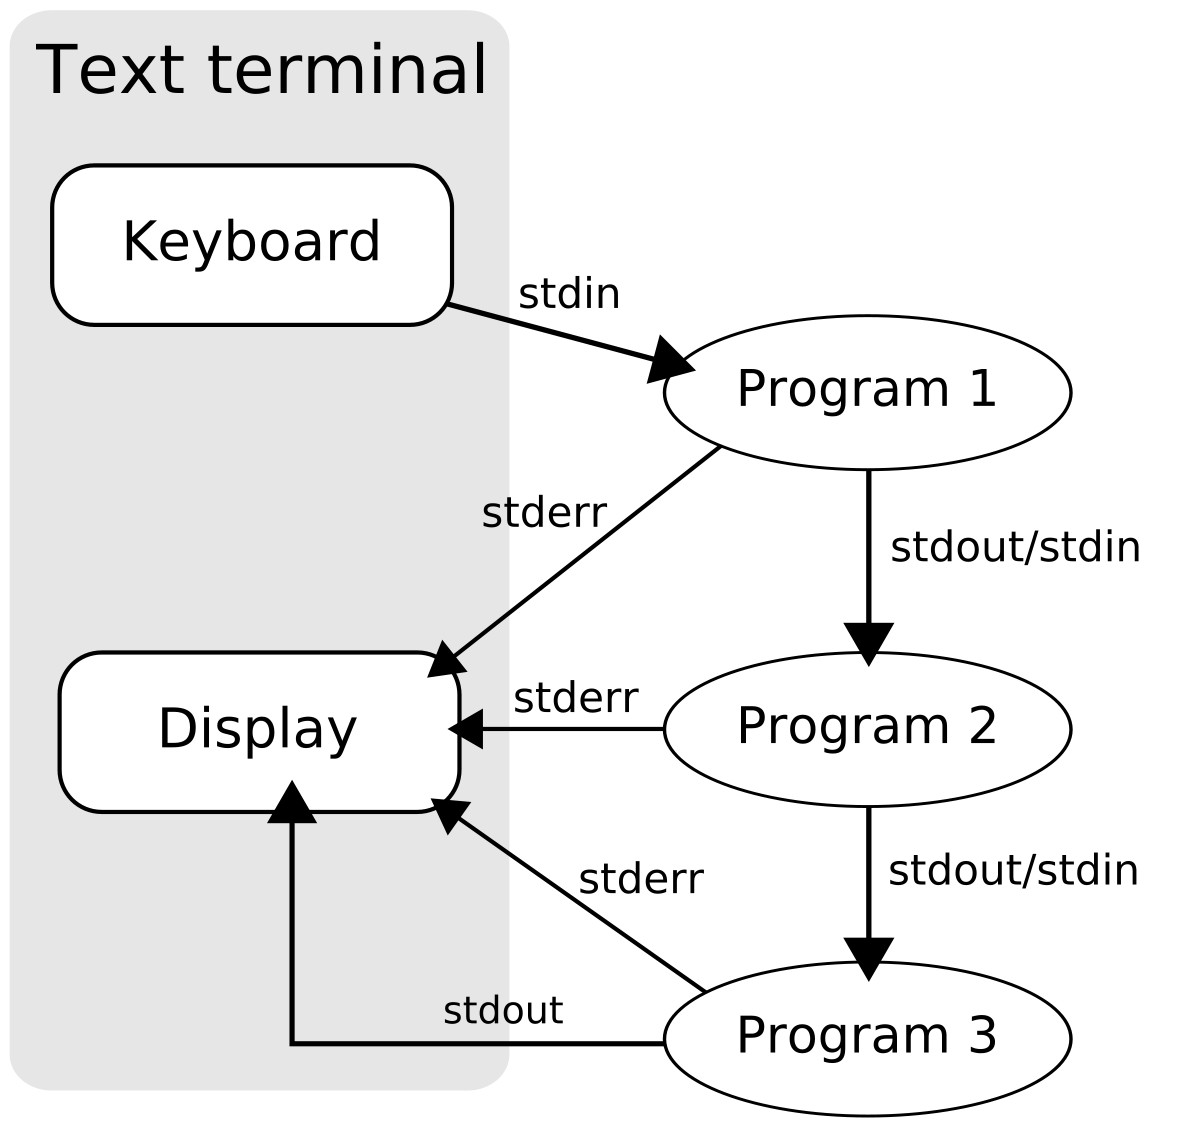
\includegraphics{pipes}
  \caption{Pipes}
  \labfig{pipes}
\end{marginfigure}

Pipes are the holy grail of Unix-like operating systems.
They are the most important concept to understand
in Unix-like operating systems.

\begin{definition}[Pipe]
  A \textbf{pipe} is a way to connect the standard output of one process
  to the standard input of another process. This is done by using the
  \lstinline||| operator.
\end{definition}

Think of the shell as a factory, and the commands as machines in the
factory. Pipes are like conveyor belts that connect the machines.
It would be a pain if we had to manually collect the produce of one
machine and then feed it to the next machine. Conveyors make it easy
by automatically taking the output of one machine and feeding it to
the next machine.

Pipes are the same, but for processes in shell.

\begin{lstlisting}[language=bash]
$ date
Thu Jul  4 09:05:30 AM IST 2024
$ date | wc
      1       7      32
\end{lstlisting}

\subsection{UNIX Philosophy}

Each process simply takes the standard input and writes to the standard
output. How those streams are connected is not the concern of the process.
This way of simply doing one thing and doing it well is the Unix philosophy
\sidenote{
The Unix philosophy, originated by Ken Thompson,
is a set of cultural norms and philosophical approaches
to minimalist, modular software development.
It is based on the experience of leading developers
of the Unix operating system.
Read more
\href{https://en.wikipedia.org/wiki/Unix\_philosophy}{online}.
}
which says that each program should do one thing and do it well.
Each process should take input from the standard input and write to
the standard output. The output of the process should be easy to
parse by another process. The output of the process should not contain
unnecessary information. This makes it easy to chain commands together
using pipes.

\subsection{Multiple Pipes}

There is no limit to the number of pipes that can be chained together.
It simply means that the output of one process is fed to the input
of the next process. This simple but powerful construct lets the user
do any and all kinds of data processing.

Imagine you have a file which contains a lot of words, you want to
find which word is present the most number of times. You can either
write a program in C or Python, etc., or you can use the power of
pipes to do it in a single line using simple GNU coreutils.

I have a file \lstinline|alice_in_wonderland.txt| which contains the
entire text of the book Alice in Wonderland. I want to find the words
that are present the most number of times.

There are some basic preprocessing you would do even if you were writing
a program. You would convert all the words to lowercase, and remove
any punctuation. This can be done using the \lstinline|tr| command.
Then you would split the text into each word. This can be done using
the \lstinline|tr| command. Then you would find the count of each word.
There are two ways of doing this, either you can use a dictionary
\sidenote{
  A dictionary in python is a hash map. It is a data structure that
  maps keys to values. The keys are unique, and the values can be
  accessed using the keys. It has amortized constant time complexity
  for insertion, deletion, and lookup.
}
to store the frequency of each word, and increase it as you iterate
over the entire text once. Or you can first sort the words, then
simply count the number of times each word is repeated. Since repeated
words would always be consecutive, you can simply count the number
of repeated words without having to store the frequency of each word.
This can be done using the \lstinline|sort| and \lstinline|uniq| commands.
Finally, you would sort the words based on the frequency and print
the top 10 words. This can be done using the \lstinline|sort| and \lstinline|head|
commands.

Lets see how we actually do this using pipes.

\begin{lstlisting}[language=bash]
$ ls alice_in_wonderland.txt
alice_in_wonderland.txt
$ tr 'A-Z' 'a-z' < alice_in_wonderland.txt  | tr -cd 'a-z ' | tr ' ' '\n' | grep . | sort | uniq -c | sort -nr | head
   1442 the
    713 and
    647 to
    558 a
    472 she
    463 it
    455 of
    435 said
    357 i
    348 alice
\end{lstlisting}

Let's go over each command one by one and see what it does.

\textbf{tr 'A-Z' 'a-z'}

\lstinline|tr| is a command that translates characters. The first argument
is the set of characters to be translated, and the second argument is
the set of characters to translate to. Here, we are translating all
uppercase letters to lowercase.
This command converts all uppercase letters to lowercase. This is done
to make the words case-insensitive.

\begin{lstlisting}[language=bash]
$ tr 'A-Z' 'a-z' < alice_in_wonderland.txt  | head -n20
alice's adventures in wonderland

                alice's adventures in wonderland

                          lewis carroll

               the millennium fulcrum edition 3.0




                            chapter i

                      down the rabbit-hole


  alice was beginning to get very tired of sitting by her sister
on the bank, and of having nothing to do:  once or twice she had
peeped into the book her sister was reading, but it had no
pictures or conversations in it, `and what is the use of a book,'
\end{lstlisting}

\begin{remark}
  Since the text is really big, I am  going to filter all the
  intermediate outputs also through the \lstinline|head| command.
\end{remark}

\textbf{tr -cd 'a-z '}

The \lstinline|-c| option is used to complement the set of characters.
The \lstinline|-d| option is used to delete the characters. Here, we are
telling the \lstinline|tr| command to delete all characters except lowercase
letters and spaces. This is done to remove all punctuation and special
characters. Observe the difference in output now.

\begin{lstlisting}[language=bash]
$ tr 'A-Z' 'a-z' < alice_in_wonderland.txt  | tr -cd 'a-z ' | head -c500
alices adventures in wonderland                alices adventures in wonderland                          lewis carroll               the millennium fulcrum edition                             chapter i                      down the rabbithole  alice was beginning to get very tired of sitting by her sisteron the bank and of having nothing to do  once or twice she hadpeeped into the book her sister was reading but it had nopictures or conversations in it and what is the use of a bookthought alice w
\end{lstlisting}

\begin{remark}
  After we have removed all the punctuation, the text is now
  only a single line. This is because we have removed all the
  characters, including the newline characters.
  Thus to restrict the output, I am using the \lstinline|head -c500|
  instead of \lstinline|head -n20|.
\end{remark}

\textbf{tr ' ' '\textbackslash n'}

The \lstinline|tr| command is used to translate characters. Here, we are
translating spaces to newline characters. This is done to split the
text into words. We are doing this so that each word is on a new line.
This is helpful as the sort and uniq commands work on lines.

\begin{lstlisting}[language=bash]
$ tr 'A-Z' 'a-z' < alice_in_wonderland.txt  | tr -cd 'a-z ' | tr ' ' '\n' | head -20
alices
adventures
in
wonderland















alices
\end{lstlisting}

\textbf{grep .}

Now we have each word on a new line.
But observe that there are many empty lines.
This is because of the multiple spaces between words and spaces around
punctuation. We can remove these empty lines using the \lstinline|grep .|
command.
\sidenote{
  We will learn more about regular expressions in the \refch{regex} chapter.
}

\begin{lstlisting}[language=bash]
$ tr 'A-Z' 'a-z' < alice_in_wonderland.txt  | tr -cd 'a-z ' | tr ' ' '\n' | grep . | head -20
alices
adventures
in
wonderland
alices
adventures
in
wonderland
lewis
carroll
the
millennium
fulcrum
edition
chapter
i
down
the
rabbithole
alice
\end{lstlisting}

Now we are almost there. We have each word on a new line. Now we can
pass this entire stream of words to the \lstinline|sort| command, this
will sort the words.

\textbf{sort}

Sort by default sorts the words in lexicographical order. This is
useful as repeated words would be consecutive. This is important
as the \lstinline|uniq| command only works on consecutive lines only.

\begin{lstlisting}[language=bash]
$ tr 'A-Z' 'a-z' < alice_in_wonderland.txt  | tr -cd 'a-z ' | tr ' ' '\n' | grep . | sort | head -20
a
a
a
a
a
a
a
a
a
a
a
a
a
a
a
a
a
a
a
a
\end{lstlisting}

If you run the command yourself without the \lstinline|head| command, you
can see that the words are sorted. The repeated words are consecutive.
In the above output we can see that the word \lstinline|a| is repeated
many times. Now we can use the \lstinline|uniq| command to count the
number of times each word is repeated.

\textbf{uniq -c}

The \lstinline|uniq| command is used to remove consecutive duplicate lines.
However, it also can count the number of times each line is repeated
using the \lstinline|-c| option.

\begin{lstlisting}[language=bash]
$ tr 'A-Z' 'a-z' < alice_in_wonderland.txt  | tr -cd 'a-z ' | tr ' ' '\n' | grep . | sort | uniq -c | head -20
    558 a
      1 abarrowful
      1 abat
      1 abidefigures
      1 able
     79 about
      1 aboutamong
      1 aboutand
      1 aboutby
      3 abouther
      3 aboutit
      1 aboutthis
      1 abouttrying
      2 above
      1 abranch
      1 absenceand
      2 absurd
      1 acceptance
      2 accident
      1 accidentally
\end{lstlisting}

Great! Now we have the count of each word. However, the words are
still sorted by the word. We want to sort the words by the count
of the word. This can be done using the \lstinline|sort| command.

\textbf{sort -nr}

Sort by default sorts in lexicographical order. However, we want to
sort by the count of the word. The \lstinline|-n| option is used to sort
the lines numerically. The \lstinline|-r| option is used to sort in
reverse order.

\begin{exercise}
  Try to run the same command without the \lstinline|-n| option.
  Observe how the sorting makes sense alphabetically, but not
  numerically.
\end{exercise}

\begin{lstlisting}[language=bash]
$ tr 'A-Z' 'a-z' < alice_in_wonderland.txt  | tr -cd 'a-z ' | tr ' ' '\n' | grep . | sort | uniq -c | sort -nr | head -20
   1442 the
    713 and
    647 to
    558 a
    472 she
    463 it
    455 of
    435 said
    357 i
    348 alice
    332 you
    332 in
    313 was
    241 that
    237 as
    202 her
    190 at
    169 on
    161 all
    158 with
\end{lstlisting}

Finally, we have the top 20 words in the file \lstinline|alice_in_wonderland.txt|
along with the count of each word.

Although the above command is a single line
\sidenote{
  Such commands are called one-liners.
}
, it is doing a lot of
processing. Still, it is very readable. This is the power of pipes.

\begin{remark}
  Usually, when we come across such one-liners, it may initially
  seem too complicated to understand. The key to understanding such
  one-liners is to break them down into smaller parts and understand
  them one component at a time from left to right. Feel free to
  execute each command separately and observe the output like we
  did above.
\end{remark}

\subsection{Piping Standard Error}

Pipes are used to connect the standard output of one process to the
standard input of another process. However, the standard error is not
connected and remains mapped to the terminal. This is because the
standard error is a separate stream from the standard output.

However, we can connect the standard error to the standard input of
another process using the \lstinline|2>\&1| operator. This is useful when
we want to process the error messages of a command.

\begin{lstlisting}[language=bash]
$ ls -d /home /nonexistant | wc
"/nonexistant": No such file or directory (os error 2)
      1       1       6
$ ls -d /home /nonexistant 2>&1 | wc
      2      10      61
\end{lstlisting}

This is same as redirecting both the streams to a single file as
demostrated earlier.

However, there is a shorter way to do this using the \lstinline||\&|
syntactic sugar.

\begin{lstlisting}[language=bash]
$ ls -d /home /nonexistant |& wc
      2      10      61
\end{lstlisting}

This does the exact same thing as \lstinline|2>\&1| followed by the pipe.

\subsection{Piping to and From Special Files}

As we discussed earlier, there are some special files in the \lstinline|/dev|
directory.

\textbf{/dev/null}

The \lstinline|/dev/null| file is a special file that discards all the data
that is written to it. It is like a black hole. All the data that is
not needed can be written to this file. Usually errors are written to
the \lstinline|/dev/null| file.

\begin{lstlisting}[language=bash]
$ ls -d /nonexistant /home 2> /dev/null
/home
\end{lstlisting}

The error is not actually stored in any file, thus the storage
space is not wasted.

\textbf{/dev/zero}

The \lstinline|/dev/zero| file is a special file that provides an infinite
stream of null bytes. This is useful when you want to provide an infinite
stream of data to a process.

\begin{lstlisting}[language=bash]
$ head -c1024 /dev/zero > zero.txt
$ ls -lh zero.txt
-rw-r--r-- 1 sayan sayan 1.0K Jul  4 15:04 zero.txt
\end{lstlisting}

Here we are taking the first 1024 bytes from the \lstinline|/dev/zero|
and writing it to the file \lstinline|zero.txt|. The file \lstinline|zero.txt|
is 1.0K in size. This is because the \lstinline|/dev/zero| file provides
an infinite stream of null bytes, of which $1024$ bytes are taken.

\begin{warn}
  Make sure to always use \lstinline|head| or any other limiter when
  working with \lstinline|/dev/zero| or \lstinline|/dev/random| as they
  are infinite streams. Forgetting this can lead to the disk being
  filled up. Head with the default parameter will also not work,
  since it depends on presence of newline characters, which is
  not there in an infinite stream of zeros. That is why we are
  using a byte count limiter using the \lstinline|-c| option.
  If you forget to add the limiter, you can press \lstinline|Ctrl+C|
  as quickly as possible to stop the process and then remove the
  file using \lstinline|rm|.
\end{warn}

\textbf{/dev/random and /dev/urandom}

The \lstinline|/dev/random| and \lstinline|/dev/urandom| files are special
files that are infinite suppliers of random bytes. The \lstinline|/dev/random|
file is a blocking random number generator. This means that it will
block if there is not enough entropy. The \lstinline|/dev/urandom| file
is a non-blocking random number generator. This means that it will
not block even if there is not enough entropy. Both can be used to
generate random numbers.

\begin{lstlisting}[language=bash]
$ head -c1024 /dev/random > random.txt
$ ls -lh random.txt
-rw-r--r-- 1 sayan sayan 1.0K Jul  4 15:04 random.txt
\end{lstlisting}

Observe that here too the file is of size 1.0K. This is because we
are still taking only the first 1024 bytes from the infinite stream
of random bytes. However, if we gzip the data, we can see that the
zeros file is much smaller than the random file.

\begin{lstlisting}[language=bash]
$ gzip random.txt zero.txt
$ ls -lh random.txt.gz zero.txt.gz
-rw-r--r-- 1 sayan sayan 1.1K Jul  4 15:11 random.txt.gz
-rw-r--r-- 1 sayan sayan   38 Jul  4 15:10 zero.txt.gz
\end{lstlisting}

The random file is 1.1K in size, while the zero file is only 38 bytes
in size. This is because the random file has more entropy and thus
cannot be compressed as much as the zero file.

\subsection{Named Pipes}

A \textbf{named pipe} is a special file that provides a way to connect
the standard output of one process to the standard input of another
process. This is done by creating a special file in the filesystem.
We have already covered named pipes in the \refch{basic} chapter.

Although a pipe is faster than a named pipe, a named pipe can be used
to connect processes that are not started at the same time or from
the same shell. This is because a named pipe is a file in the filesystem
and can be accessed by any process that has the permission to access
the file.

Try out the following example. First create a named pipe using the
\lstinline|mkfifo| command.

\begin{lstlisting}[language=bash]
$ mkfifo pipe1
\end{lstlisting}

Then run two processes, one that writes to the named pipe, another
that reads from the named pipe. The order of running the processes
is not important.

\textbf{Terminal 1:}
\begin{lstlisting}[language=bash]
$ cat /etc/profile > pipe1
\end{lstlisting}

\textbf{Terminal 2:}
\begin{lstlisting}[language=bash]
$ wc pipe1
     47     146     993 pipe1
\end{lstlisting}

\begin{exercise}
  After you have created the named pipe,
  try changing the order of running the other two processes.
  Observe that whatever is run first will wait for
  the other process to start.
  This is because a named pipe is not storing the data piped to it
  in the filesystem. It is simply a buffer in the memory.
\end{exercise}

A named pipe is more useful over regular files when two processes
want to communicate with each other. This is because a named pipe
is

\begin{enumerate}
  \item Faster than a regular file as it does not store the data in
    the file system.
  \item Independent of the order of launching the processes.
    The reader can be launched first and it will still wait for
    the writer to send the data.
  \item Works concurrently. The writer does not need to be done
    writing the entire data before the reader can start reading.
    The reader can start as soon as the writer starts writing.
    The faster process will simply block until the slower process
    catches up.
\end{enumerate}

To demonstrate the last point, try running the following commands.

Ensure that a named pipe is created.

\textbf{Terminal 1:}

\begin{lstlisting}[language=bash]
$ grep linux pipe1
\end{lstlisting}

This process is looking for lines containing the word \lstinline|linux|
in the file \lstinline|pipe1|. Initially it will simply block.
Grep is a command that does not wait for the entire file to be read.
It starts printing output as soon as a line containing the pattern
is read.

\textbf{Terminal 2:}
\begin{lstlisting}[language=bash]
$ tree / > pipe1
\end{lstlisting}

This command is attempting to list out each and every file on
the filesystem. This takes a lot of time. However, since
we are using a named pipe, the \lstinline|grep| command will start
running as soon as the first line is written to the pipe.

You can now observe the first terminal will start printing
some lines containing the word \lstinline|linux| as soon as the
second terminal starts writing to the pipe.

Now try the same with a regular file.

\begin{lstlisting}[language=bash]
$ touch file1 # ensure its a normal file
$ tree / > file1
$ grep linux file1
\end{lstlisting}

Since this is a regular file, we cannot start reading from the
file before the entire file is written. If we do that, the grep
command will quit as soon as it catches up with the writer, it
will not block and wait.

Observe that to start getting output on the screen takes a lot
longer in this method. Not to mention the disk space wasted
due to this.

\begin{remark}
  Remember that when we use redirection (\lstinline|>|) to write to a file,
  the shell truncates the file. But when we use a named pipe, the shell
  knows that the file is a named pipe and does not truncate the file.
\end{remark}

\subsection{Tee Command}

The \lstinline|tee| command is a command that reads from the 
standard input and writes to the standard output and to a file.
It is very useful when you want to save the output of a command
but also want to see the output on the terminal.

\begin{lstlisting}[language=bash]
$ ls -d /home /nonexistant | tee output.txt
ls: cannot access '/nonexistant': No such file or directory
/home
$ cat output.txt
/home
\end{lstlisting}

Observe that only the standard output is written to the file, and
not the standard error. This is because pipes only connect the
standard output to the standard input of the next command, and the
standard error remains mapped to the terminal.

Thus in the above output, although it may look like that both
the standard output and the standard error are written to the
terminal by the same command, it is not so.

The standard error of the ls command remains mapped to the terminal,
and thus gets printed directly, whereas the standard output is
redirected to the standard input of the tee command, which then
prints that to the standard output (and also writes it to the file).

You can also mention multiple files to write to.

\begin{lstlisting}[language=bash]
$ ls -d /home | tee output1.txt output2.txt
$ cat output1.txt
/home
$ cat output2.txt
/home
$ diff output1.txt output2.txt
$
\end{lstlisting}

\begin{remark}
  The \lstinline|diff| command is used to compare two files. If the
  files are the same, then the \lstinline|diff| command will not print
  anything. If the files are different, then the \lstinline|diff| command
  will print the lines that are different.
\end{remark}

We can also append to the file using the \lstinline|-a| option.

\begin{lstlisting}[language=bash]
$ ls -d /home | tee output.txt
$ ls -d /etc | tee -a output.txt
$ cat output.txt
/home
/etc
\end{lstlisting}

\section{Command Substitution}

We have already seen that we can run multiple commands in a subshell
in bash by enclosing them in parentheses.

\begin{lstlisting}[language=bash]
$ (whoami; date)
sayan
Thu Jul  4 09:05:30 AM IST 2024
\end{lstlisting}

This is useful when you simply want to print the standard output of the
commands to the terminal. However, what if you want to store the output
of the commands in a variable? Or what if you want to pass the standard
output of the commands as an argument to another command?

To do this, we use command substitution. Command substitution is a way
to execute one or more processes in a subshell and then use the output
of the subshell in the current shell.

There are two ways to do command substitution.

\begin{enumerate}
  \item Using backticks \lstinline|`command`| - this is the legacy way
    of doing command substitution. It is not recommended to use this
    as it is difficult to read and can be confused with single quotes.
    It is also harder to nest.
  \item Using the \lstinline|$(command)| syntax - this is the recommended
    way of doing command substitution. It is easier to read and nest.
\end{enumerate}

\marginnote{
  Throughout this book, we will use the \lstinline|$(command)| syntax
  and not the backticks.
}

\begin{lstlisting}[language=bash]
$ echo "Today is $(date)"
Today is Thu Jul  4 09:05:30 AM IST 2024
\end{lstlisting}

Here we are using the \lstinline|$(date)| command substitution to get
the current date and time and then using it as an argument to the
\lstinline|echo| command.

\begin{lstlisting}[language=bash]
$ myname="$(whoami)"
$ mypc="$(hostname)"
$ echo "Hello, $myname from $mypc"
Hello, sayan from rex
\end{lstlisting}

We can store the output of the command in a variable and then use
it later. This is useful when you want to use the output of a command
multiple times.

\begin{remark}
  Although you do not need to use the quotes with the command substitution
  in this case, it is always recommended to use quotes around the variable
  assignment, since if the output is multiword or multiline, it will
  throw an error.
\end{remark}

\section{Arithmetic Expansion}

Arithmetic expansion allows the evaluation of an arithmetic
expression and the substitution of the result. The format for
arithmetic expansion is:

\begin{lstlisting}[language=bash]
$(( expression ))
\end{lstlisting}

This is the reason we cannot directly nest subshells without a
command between the first and the second subshell.

\begin{lstlisting}[language=bash]
$ cat /dev/random | head -c$((1024*1024)) > random.txt
$ ls -lh random.txt
-rw-r--r-- 1 sayan sayan 1.0M Jul  4 15:04 random.txt
\end{lstlisting}

Here we are using \textbf{arithmetic expansion} to calculate the
number of bytes in 1MiB
\sidenote{
  $1$MiB $= 1024$KiB $= 1024\times 1024$ bytes
  - this is called a mebibyte \\
  $1$MB $= 1000$KB $= 1000\times 1000$ bytes
  - this is called a megabyte \\
  This is a very common confusion amongst common people.
  Kilo, Mega, Giga are SI prefixes,
  while Kibi, Mebi, Gibi are IEC prefixes.
}
and then using it as an argument to the head command.
This results in creation of a file \lstinline|random.txt| of size 1MiB.

\subsection{Using variables in arithmetic expansion}

We can also use variables in arithmetic expansion.
We dont have to use the \lstinline|$| operator to access the value of
the variable inside the arithmetic expansion.

\begin{lstlisting}[language=bash]
$ a=10
$ b=20
$ echo $((a+b))
30
\end{lstlisting}

There are other ways to do arithmetic in bash, such as using the
\lstinline|expr| command, or using the \lstinline|let| command. However,
the \lstinline|$(())| syntax is the most recommended way to do simple
arithmetic with variables in bash.

\section{Process Substitution}

Process substitution is a way to provide the output of a process
as a file. This is done by using the \lstinline|<(command)| syntax.

Some commands do not accept standard input. They only accept
a filename as an argument. This is the exact opposite of the
issue we had with the \lstinline|read| command, which accepted
only standard input and not a filename. There we used the
\lstinline|<| operator to redirect the standard input from a file.

The \lstinline|diff| command is a command that compares two files
and prints out differences. It does not accept standard input.
If we want to compare differences between the output of two
processes, we can use process substitution.

Imagine you have two directories and you want to compare the
files in the two directories. You can use the \lstinline|diff|
command to compare the two directories.

\begin{lstlisting}[language=bash]
$ ls
$ dir1 dir2
$ ls dir1
file1 file2 file3
$ ls dir2
file2 file3 file4
\end{lstlisting}

We can see that the two directories have some common files
(\lstinline|file2| and \lstinline|file3|) and some different files
(\lstinline|file1| in dir1 and \lstinline|file4| in dir2).

However, if we have a lot of files, it is difficult to see
manually which files are different.

Let us first try to save the output of the two \lstinline|ls|
commands to files and then compare the files using diff.

\begin{lstlisting}[language=bash]
$ ls
dir1 dir2
$ ls dir1 > dir1.txt
$ ls dir2 > dir2.txt
$ diff dir1.txt dir2.txt
1d0
< file1
3a3
> file4
\end{lstlisting}

Great! We can see that the file \lstinline|file1| is present only
in \lstinline|dir1| and the file \lstinline|file4| is present only
in \lstinline|dir2|. All other files are common.

However observe that we had to create two files \lstinline|dir1.txt|
and \lstinline|dir2.txt| to store the output of the \lstinline|ls|
commands. This is not efficient. If the directories contained
a million files, then we would have to store tens or
hundreds of megabytes of data in the files.

It sounds like a job for the named pipes we learnt earlier.
Lets see how easier or harder that is.

\begin{lstlisting}[language=bash]
$ ls
dir1 dir1.txt dir2 dir2.txt
$ rm dir1.txt dir2.txt
$ mkfifo dir1.fifo dir2.fifo
$ ls dir1 > dir1.fifo &
$ ls dir2 > dir2.fifo &
$ diff dir1.fifo dir2.fifo
1d0
< file1
3a3
> file4
\end{lstlisting}

Et voila! We have the same output as before, but without the
data actually being stored in the filesystem. The data is
simply stored in the memory till the \lstinline|diff| command
reads it. However observe that we had to create two named
pipes, and also run the ls processes in the background as
otherwise they would block.
Also, we have to remember to delete the named pipes after
using them.
This is still too much hassle.

Let us remove the named pipes and the files.
\begin{lstlisting}[language=bash]
$ rm *fifo
\end{lstlisting}

Now let us see how easy it is using process substitution.

\begin{lstlisting}[language=bash]
$ diff <(ls dir1) <(ls dir2)
1d0
< file1
3a3
> file4
\end{lstlisting}

Amazing! We have the same output as before, but without having
to initialize anything. The process substitution does all the
magic of creating temporary named pipes and running the processes
with the correct redirections concurrently. It then substitutes
the filenames of the named pipes in the place of the process
substitution.

Process substitution is also extremely useful when comparing
between expected output and actual output in some evaluation
of a student's scripts.
\sidenote{
  Try to find if this is used in the evaluation scripts
  of the VM Tasks!
}

We can also use process substitution to provide input to a process
running in the subshell.

\begin{lstlisting}[language=bash]
tar cf >(bzip2 -c > file.tar.bz2) folder1
\end{lstlisting}

This calls \lstinline|tar cf /dev/fd/?? folder1|,
and \lstinline|bzip2 -c < /dev/fd/?? > file.tar.bz2|.
\sidenote{
  Here I have used \lstinline|??| as the file descriptor number.
  In actuality, the file descriptor number will be a number that is not already in use.
}

\marginnote{
  This example is lifted from
  \url{https://tldp.org/LDP/abs/html/process-sub.html}.
  If you are interested in more examples of process substitution,
  refer the same.
}

Because of the \lstinline|/dev/fd/<n>| system feature,
the pipe between both commands does not need to be named.
This can be emulated as

\begin{lstlisting}[language=bash]
mkfifo pipe
bzip2 -c < pipe > file.tar.bz2 &
tar cf pipe folder1
rm pipe
\end{lstlisting}

\begin{remark}
  tar is a command that is used to create archives.
  It simply puts all the files and directories in a single file.
  It does not perform any compression. The \lstinline|c| option is
  used to create an archive. The \lstinline|f| option is used to
  mention the name of the archive. The \lstinline|bzip2| command
  is used to compress files. The \lstinline|-c| option is used to
  write the compressed data to the standard output. The \lstinline|>|
  operator is used to redirect the standard output to a file.
  We will cover tar and zips in more detail later.
\end{remark}

That is pretty much all you need to know about pipes and redirections.
To really understand and appreciate the power of pipes and redirections,
you have to stop thinking imperically (like C or Python) and start
thinking in streams, like a functional programming language.
Once this paradigm shift happens, you will start to see the power
of pipes and redirections and will be able to tackle any kind of
task in the command line.

\vfill
\pagebreak
\section{Summary}

Let us quickly summarize the important syntax and commands we learnt
in this chapter.

\begin{table*}[h!]
  \caption{Pipes, Streams, and Redirection syntax}
  \labtab{pipesyntax}
  \begin{tabular}{c c l}
    \toprule
    \lstinline|Syntax| & \lstinline|Command| & \lstinline|Description| \\
    \midrule
    \lstinline|;| & Command Separator & Run multiple commands\\ & & in a single line\\
    \lstinline|&&| & Logical AND & Run the second command only \\ & & if the first command succeeds\\
    \lstinline|||| & Logical OR & Run the second command \\ & & only if the first command fails\\
    \lstinline|>| & Output Redirection & Redirect the stdout of \\ & & the process to a file\\
    \lstinline|>>| & Output Redirection & Append the stdout of the \\ & & process to a file\\
    \lstinline|<| & Input Redirection & Redirect the stdin of \\ & & the process from a file\\
    \lstinline|2>| & Error Redirection & Redirect the stderr of \\ & & the process to a file\\
    \lstinline|2>\&1| & Error Redirection & Redirect the stderr of the \\ & & process to the stdout\\
    \lstinline|<<EOF| & Here Document & Redirect the stdin of \\ & & the process from a block of text\\
    \lstinline|<<<| & Here String & Redirect the stdin of \\ & & the process from a string\\
    \lstinline||| & Pipe & Connect the stdout of one process \\ & & to the stdin of another process\\
    \lstinline||\&| & Pipe Stderr & Connect the stderr of one process \\ & & to the stdin of another process\\
    \lstinline|$(command)| & Command Substitution & Run a command and use \\ & & the output in the current shell\\
    \lstinline|$((expression))| & Arithmetic Expansion & Evaluate an arithmetic \\ & & expression\\
    \lstinline|<(command)| & Process Substitution & Provide the output of \\ & & a process as a file\\
    \lstinline|>(command)| & Process Substitution & Provide the input to a \\ & & process from a file\\
    \bottomrule
  \end{tabular}
\end{table*}
